\subsection{MOSFET Structure and basic function}

The purpose of this section is only to apply the hydraulic intuition to the transistor, by studying its structure and basic function. The details of the operation of transistors are significantly more complex than what we will cover here, and most of the necessary details will be covered in the next chapter.  

\begin{figure}[H]
    \centering
    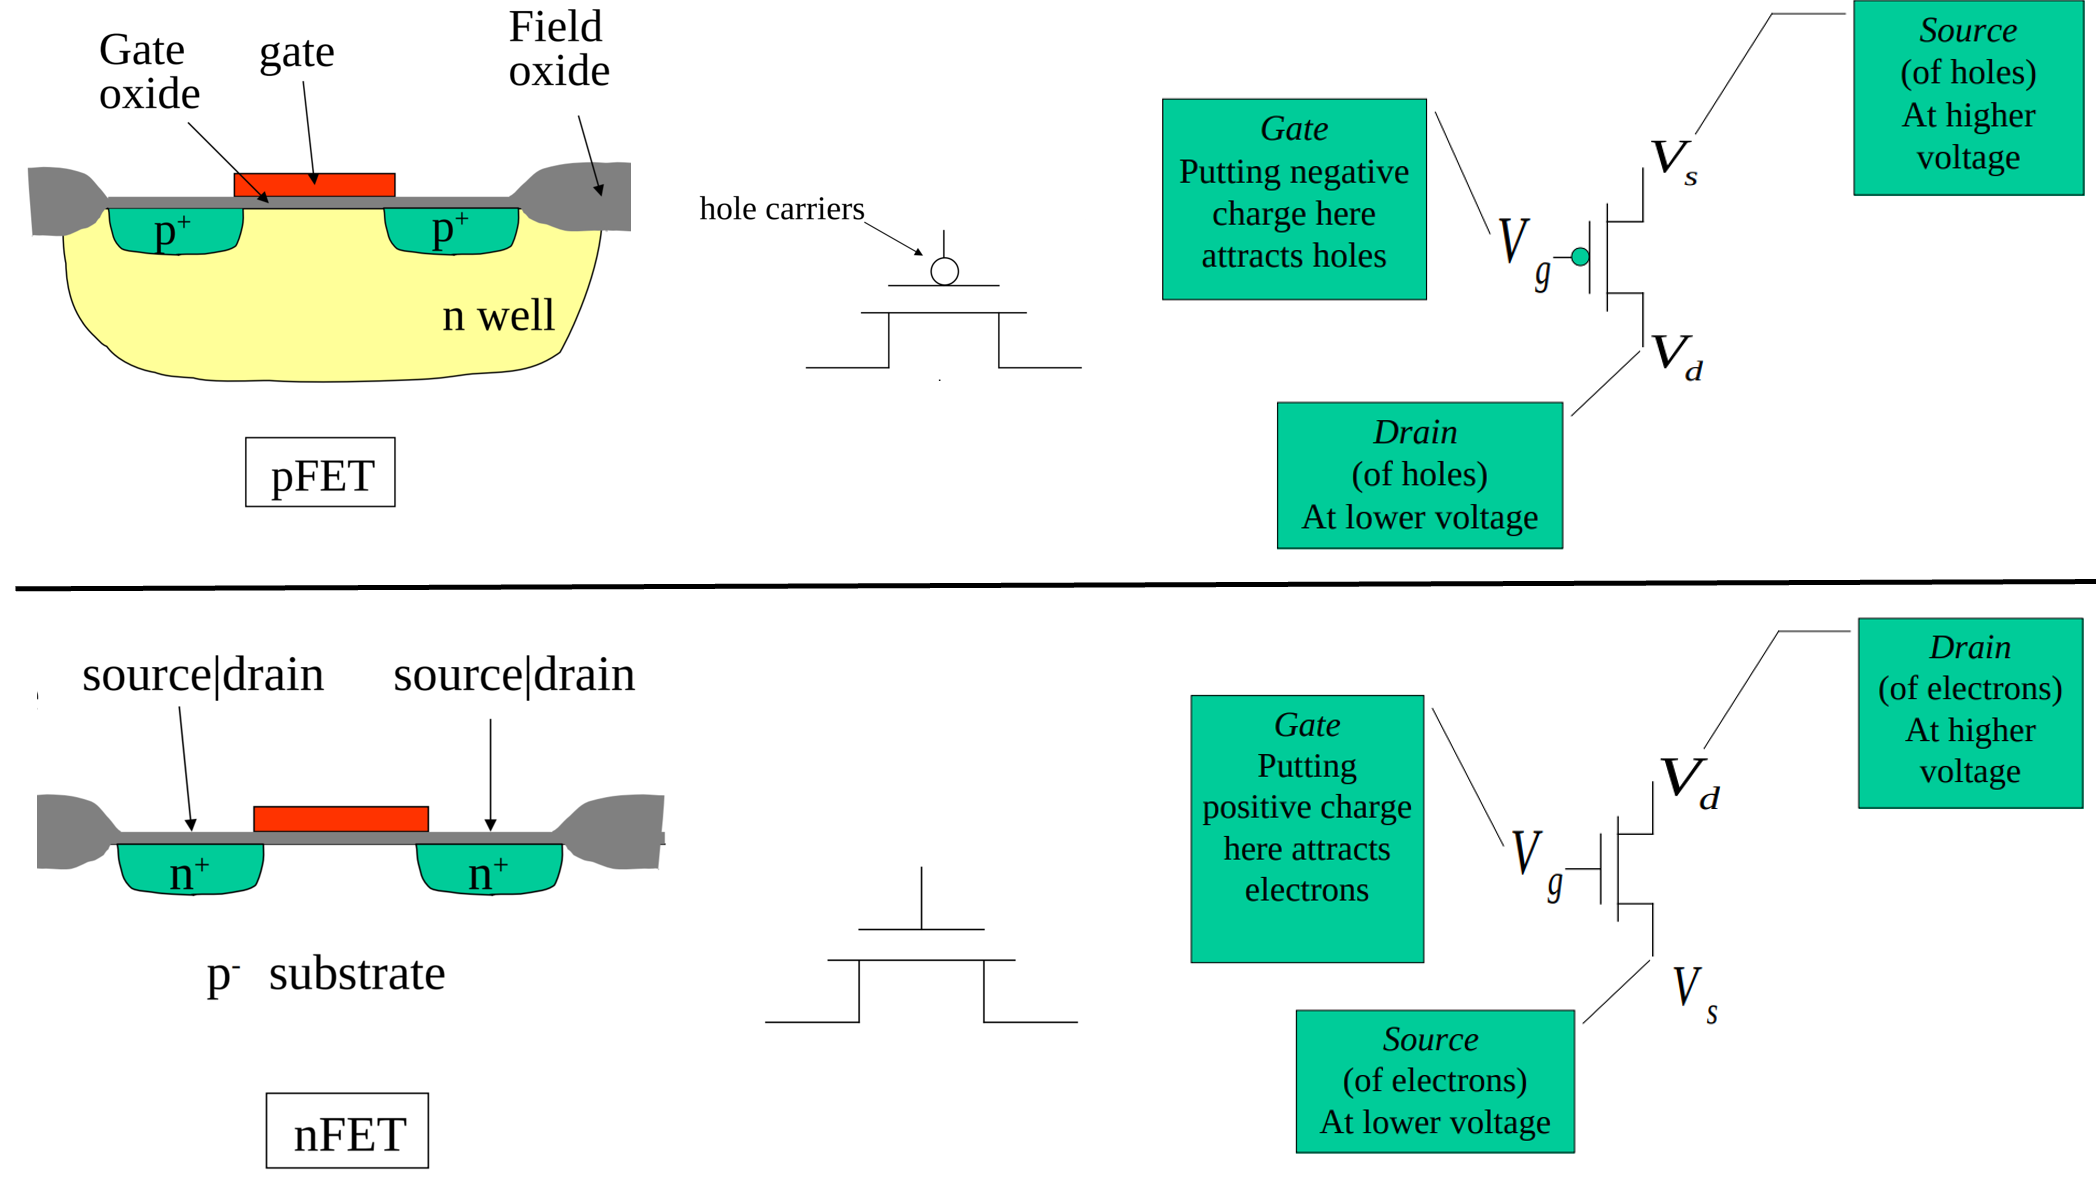
\includegraphics[width=1\linewidth]{../../Figures/The_Transistor.PNG}
    \caption{Essential structural and schematic description of the two transistor type: the pFET and nFET. On the left, structure. In the middle, circuit schematic. On the right, principle of the 3 operating points. Adapted from lecture notes}
    \label{fig:The Transistor}
\end{figure}


\textbf{NEED TO INCLUDE THE IDEA OF TRANSISTOR WIDTH AND LENGTH, AS WELL AS THE FIGURE SLIDE 23 IN 2B MOSFET LECTURE ABOUT TRANSISTOR MIS STRUCTURE}


There are two distinct types of MOSFETs: the pFET and the nFET. While they use the same principle of operation, some basic differences should be noted. There exists also other type of practical operation differences that we will look at later.

Both the pFET and the nFET have 4 terminals, and 3 of main interest. That is, they both possess a \textbf{source, drain and gate}. The source and drain are pieces of doped silicon - p-type doped in the case of pFETs and n-type doped in the case of nFETs. You can see in the schematic $p^+$ and $n^+$ for the source and drain terminals, with the $+$ indicating the doping concentration. Typically, both source and drain have the same doping concentration, but more on this later. In both the pFET and nFET, the source and drain are in contact with a \textbf{well or substrate} (take them as representing the same thing for now) of opposite type. That is, the n-type doped silicon source and drain in an N-FET are in sitting on p-type doped silicon well. This should ring a bell: we're dealing with PN-Junctions!  

We do \textbf{not} want to have current flowing from the the source and/or drain to the well, we actually want it to stay still (for now) - so we \textbf{reverse bias} the PN-Junction! That is, in a nFET, we apply a \textit{lower} potential on the p-well then on the source and drain, and vice verca in a pFET \footnote{No potential difference between source and well is actually okay, so you either need lower (or higher in the case of pFET) potential differerence or no potential difference at all to keep this reverse bias.}. You should see clearly why this yields a reverse bias function, and a subsequent \textbf{depletion region}. \footnote{If you don't see this clearly, I suggest reviewing the section on PN-Junctions, as well will continue building from this in the next bits!}

Now what about the gate? The gate is a piece of conducting metal, and it is separated from the source, drain and well with a \textbf{gate oxide}. This is an insulator material. This should also ring a bell: conductive materials separated by an insulator - we're dealing with some capacitor! More on this later.  

On the nFET diagram, you may have noticed "source/drain" on both terminals. This also holds for the pFET. Essentially, the transistor is a perfectly symmetric device, and both terminals can be used as source or drain. Now let's look at what exactly is the difference between source and drain.

\paragraph{Source and drain: what's the difference?} Remember from the hydraulic analogy that our source and drain of water had some potential difference. This is exactly what happens in the transistor, and this potential difference will determine what is the source and what is the drain. Things have the same logic, but in reverse, for the pFET and nFET: this is showed on the right hand side of figure \ref{fig:The Transistor}. In an pFET, the source is at the node at the highest voltage. We call this $V_s$ for \textit{source voltage}. The \textit{drain voltage} $V_d$ is at a lower potential. Remember that this is not the same as the doping concentration - and we'll get to that soon. If we choose to apply the highest voltage on the right terminal of the pFET, this becomes the source and the other becomes the drain, and vice versa. Again, it is symmetric and its operation depends on the voltage difference between the source and drain. This voltage difference has a specific name: \textbf{drain to source voltage}, and is note $V_{ds}$ it is simply the difference between the two: $V_d - V_s$. In the case of the nFET, it's exactly the opposite. The source is at the lowest potential and the drain at higher potential. This should make sense intuitively: in a pFET, charge carriers are positive holes, there are more in higher voltage points, which thus make them the source - they travel to the drain at lower potential. In a nFET, charge carriers are negative electrons, there are more electrons in the lower voltage points, which thus make them the source - they travel to the drain at higher potential. 

\paragraph{Circuit diagram} Both diagrams of the pFET and nFET are built around the same structure, except that the pFET has a small circle between its gate and the line. This symbolizes the holes, as opposed to electrons, which are the charge carriers in a pFET (as the source and drain are p-type doped silicon).

\paragraph{The gate} Now that we conceptually explained the difference between the source and the drain, we need to look at the gate. Remember from the hydraulic analogy that the gate is what controls the flow of water, provided we have a potential difference between the source and the drain. The same principle applies in transistors. The dynamics are best understood schematically - and keep in mind that this is just to build an intuition!

\begin{figure}[H]
    \centering
    \includegraphics[width=1\linewidth]{../../Figures/Gate Voltage.png}
    \caption{Basic principle behind current flow when applying gate voltage. Personnal drawing, adapted from a few figures in the lecture notes.}
    \label{fig:Gate_Voltage}
\end{figure}

The above figure draws an N-FET with a $V_{ds}$ of $1V$ - so potential difference between the source and drain is present. We now apply a gate voltage $V_g = 0.5V$. Because of the positive voltage, we have a positive charges that accumulate on the gate. This naturally repels the positive charges on the p substrate (because alike charges repel each other) and creates some kind of corridor virtually of positive charges, where negative charges start to accumulate. This corridor suddenly allows a flow of charges through diffusion between the source and the drain as we have a significant drain to source potential difference, and thus a current. This is because, in this region, we are not anymore in a standard equilibrium PN Junction configuration anymore. This region, drawn in orange on the figure is called the \textbf{depletion region}. 